\RequirePackage{mmap}
\documentclass[12pt]{article}
\usepackage[utf8]{inputenc}
\usepackage{geometry}
\geometry{
  margin=1in,
}
\usepackage{amsmath,amsthm,amssymb, listings, color, bm}
\usepackage{mathtools}
\usepackage{changepage}% http://ctan.org/pkg/changepage
\usepackage{enumitem}
\usepackage{csquotes}
\usepackage{fancyhdr}
\usepackage[T1]{fontenc}
\usepackage{titlesec}
\usepackage[absolute]{textpos}
\usepackage[hidelinks]{hyperref}
\usepackage{fontspec}
\usepackage[linesnumbered,ruled]{algorithm2e}
\setmainfont{Latin Modern Roman}
%% \usepackage{setspace}
%% \doublespacing

\renewcommand{\P}{\mathbb{P}}
\newcommand{\E}{\bm{E}}
\newcommand{\Var}{\bm{Var}}
\newcommand{\ul}[1]{\underline{#1}}

\newtheorem{theorem}{Theorem}[section]
\newtheorem{corollary}{Corollary}[theorem]
\newtheorem{lemma}[theorem]{Lemma}
\theoremstyle{definition}
\newtheorem{definition}{Definition}[section]

\DeclareMathOperator*{\argmax}{arg\,max}
\DeclareMathOperator*{\argmin}{arg\,min}

\setlength{\parindent}{0.25in}

\newif\ifextra
\extrafalse

\title{}

\pagenumbering{arabic}

\begin{document}
\pagestyle{fancy}
\fancyhf{} % sets both header and footer to nothin
\cfoot{\thepage}
\renewcommand{\headrulewidth}{1pt}
\lhead{\fontsize{10}{12} \selectfont CSE 446: Machine Learning (Prof. Sham Kakade)\\\textbf{\emph{Section 3: Perceptron, Probability, Bayesian Optimal Classifier}} }
\rhead{\fontsize{10}{12} \selectfont Kaiyu Zheng (TA)\\ \today}

This is my preperation notes for teaching in sections during the winter 2018 quarter for course CSE 446. Useful for myself to review the concepts as well.

\section{More Linear Algebra}

\begin{definition}[Dot Product]
\emph{(Algebraic definition)} Let $\bm{a}$ and $\bm{b}$ be two vectors in $\mathbb{R}^n$. Then the dot product (or inner product) between $\bm{a}$ and $\bm{b}$ is defined as:
    \begin{equation}
        \bm{a}\cdot\bm{b}=\bm{a}^T\bm{b}=\sum_{i=1}^{n}a_ib_i
    \end{equation}
    
\emph{(Geometric definition)}  The dot product of two Euclidean vectors $\bm{a}$ and $\bm{b}$ is defined by
    \begin{equation}
        \bm{a}\cdot\bm{b}=|\bm{a}||\bm{b}|cos(\theta_{\bm{a},\bm{b}})
    \end{equation}
    
Also, The dot product $\bm{w}\cdot\bm{x}=b$ is a hyperplane, where $\bm{w}$ is normal to it.
\end{definition}

\begin{definition}[Projection]
  Let $\bm{a}$ and $\bm{b}$ be two vectors in $\mathbb{R}^n$. The projection of $\bm{b}$ onto $\bm{a}$ is defined
  \begin{equation}
proj_{\bm{a}}\bm{b}=\frac{\bm{a}\cdot\bm{b}}{|\bm{a}|}\frac{\bm{a}}{|\bm{a}|}=\frac{\bm{a}\cdot\bm{b}}{|\bm{a}|^2}\bm{a}
  \end{equation}
The projection of a 2-D vector $\bm{x}$ onto a 1-D line identified by unit vector $\bm{u}$ is $(\bm{x}\cdot\bm{u})\bm{u}$. To project a $N$-D vector $\bm{x}$ down to $K$-D $\hat{\bm{x}}$, we have $\hat{\bm{x}}=\sum_{i=1}^K(\bm{x}\cdot\bm{u}_i)\bm{u}_i$.

  
\begin{definition}[Outer Product]
Let $\bm{a}$ and $\bm{b}$ be two vectors in $\mathbb{R}^n$. Then the outer product (or tensor product) between $\bm{a}$ and $\bm{b}$ is defined such that $(\bm{a}\bm{b}^T)_{ij}=a_ib_j$:
    \begin{align}
        \bm{a}\bm{b}^T&=\begin{bmatrix}
        a_1b_1 & a_1b_2 & \cdots & a_1b_n\\
        a_2b_1 & a_2b_2 & \cdots & a_2b_n\\
        \vdots & \vdots & \ddots & \vdots\\
        a_nb_1 & a_nb_2 & \cdots & a_nb_n\\
        \end{bmatrix}
    \end{align}
\end{definition}
  
\end{definition}

\subsection{Matrix Multiplication} 
Let $\bm{A}\in M_{n\times p}(\mathbb{R})$ and $\bm{B}\in M_{p\times m}(\mathbb{R})$, then $\bm{A}\bm{B}\in M_{n\times m}(\mathbb{R})$. Matrix multiplication $\bm{AB}$ can be interpreted in two ways.

\begin{enumerate}[label=\theenumi)]
    \item When we consider row vectors of $\bm{A}$ and column vectors of $\bm{B}$, the multiplication $\bm{AB}$ can be viewed as
        \begin{equation}
            \bm{A}\bm{B} =  \begin{bmatrix*}[l]
            \bm{Ab}_{|1} & \bm{Ab}_{|2} & \cdots & \bm{Ab}_{|m}\\
            \end{bmatrix*}
        \end{equation}
    where $\bm{B}=\begin{bmatrix*}[l]
        \bm{b}_{|1} & \bm{b}_{|2} & \cdots & \bm{b}_{|m}\\
        \end{bmatrix*}$. We know $(\bm{Ab}_{|k})_i=\bm{\ul{a}}_i^T\bm{b}_{|k}$. Therefore, $(\bm{AB})_{ij}=\bm{\ul{a}}_i^T\bm{b}_{|j}$.
        
    \item When we consider column vectors of $\bm{A}$ and row vectors of $\bm{B}$, the multiplication $\bm{AB}$ can be viewed as 
    \begin{equation}\label{eq:mmult_2}
        \bm{AB}=\sum_{i=1}^{p}\bm{a}_{|i}\bm{\ul{b}}_i^T
    \end{equation}
    where $\bm{a}_{|i}\bm{\ul{b}}_i^T$ is the \emph{outer product} with output dimension of $n\times m$.
\end{enumerate} 

\begin{definition}[Orthogonal Matrix]
An \emph{orthogonal matrix} $\bm{Q}$ is a square matrix with real entries whose columns and rows are orthogonal unit vectors (i.e., \emph{orthonormal} vectors), i.e.
\begin{equation}\label{eq:orthogonal}
    \bm{Q}^T\bm{Q}=\bm{Q}\bm{Q}^T=\bm{I}
\end{equation}
\end{definition}
Therefore, we have $\bm{Q}^T=\bm{Q}^{-1}$. To fully understand why Equation \ref{eq:orthogonal} holds, we need to know that for two orthogonal vectors $\bm{u_1}$ and $\bm{u_2}$, $\bm{u_1}^T\bm{u_2}=0$. And $\bm{u_1}^T\bm{u_1}=|\bm{u_1}|^2=1$. Therefore, in the resulting matrix, all entries are 0 except for ones along the diagonal.

\section{Probability}

Parts of this section reference \cite{koller2009probabilistic}.

\paragraph{Event space} We define a \emph{space} $\Omega$ to be the set of all possible outcomes. An \textbf{event space} $\mathcal{S}$ is the set of measurable \textbf{events} $\alpha$ such that $\alpha\in\mathcal{S}$ and $\alpha\subseteq\Omega$ to which we are willing to assign probabilities. For example, if we roll a dice, then $\Omega=\{1,2,3,4,5,6\}$. A possible event could be $\{1\}$ (we rolled one),  $\{1,3,5\}$ (we rolled odd), etc. We say an event $\alpha$ \emph{happened} if we observed an outcome $r\in\alpha$.  The event space $\mathcal{S}$ is closed under union ($\alpha\in\mathcal{S}\land \beta\in\mathcal{S}\rightarrow\alpha\cup\beta\in\mathcal{S}$) and complementation ($\alpha\in\mathcal{S}\rightarrow\Omega-\alpha\subseteq\mathcal{S}$).

\paragraph{Probability distribution} Given $(\Omega,\mathcal{S})$, a \textbf{probability distribution} $\P:\mathcal{S}\rightarrow\mathbb{R}$ is a mapping from events to real values, such that (1) for all $\alpha\in\mathcal{S}$, $\P(\alpha)\geq 0$, (2) $\P(\Omega)=1$, and (3) for $\beta\in\mathcal{S}$, $\P(\alpha\cup\beta)=\P(\alpha)+\P(\beta)-\P(\alpha\cap\beta)$.

\paragraph{Random variable} A random varialbe $X:\Omega\rightarrow\mathbb{R}$ associates each outcome in $\Omega$ with a value. We use $val(X)$ to denote the set of possible values that $X$ can take. Random variables can be discrete or continuous. We primarily consider discrete ones. For simplicity, if $x, y$ are generic values for random variables $X$ and $Y$, then we write $\P(X=x,Y=y)$ as $\P(X,Y)$. For a specific value $x$, we write $\P(X=x)$ as $\P(x)$.

\paragraph{Marginal distribution} The marginal distribution over random variable $X$ is $\P(X)$.

\paragraph{Joint distribution} The joint distribution over random variables $X_1,\cdots X_n$ is $\P(X_1,\cdots,X_n)$ satisfying $\P(X_1)=\sum_{x_i,\cdots x_n}\P(X_1,x_2,\cdots,x_n)$. Note that 1 is arbitrarily chosen.

\paragraph{Conditional probability} For random variables $X, Y$, $\P(X,Y)=\P(X)\P(Y|X)$, where $\P(Y|X)$ is the probability of $Y$ conditioned on $X$. For random variables $X_1,\cdots,X_n$, we have $\P(X_1,\cdots,X_n)=\P(X_1)(X_2|X_1)\P(X_3|X_1,X_2)\cdots\P(X_n|X_1,\cdots,X_{n-1})$.

\paragraph{Independence} $X$ and $Y$ are independent if $\P(X,Y)=\P(X)\P(Y)$. $X$ and $Y$ are \emph{conditionally independent} given $Z$ if $\P(X|Y,Z)=\P(X|Z)$ or $\P(X,Y|Z)=P(X|Z)P(Y|Z)$.

\paragraph{Bayes's Theorem} Because $\P(X,Y)=\P(Y)\P(X|Y)=\P(X)P(Y|X)$, we can write
\begin{equation}
  \P(X|Y) = \frac{\P(X)\P(Y|X)}{\P(Y)}
\end{equation}
where $\P(X)$ is called the prior, and $\P(X|Y)$ is called the posterior.

\paragraph{Expectation} For discrete random variable $X$, the expectation of $X$ under distribution $\P$ is defined as
\begin{equation}
  \E_{\P}[X]=\sum_{x}x\P(x)
\end{equation}
We can also write it as $\E_{X}$. Note that we can show $\E[f(X)]=\sum_{x}f(x)\P(x)$. When the subscript is not present, $\E[f(X)]=\E_{X}[f(X)]$, and $\E[f(X,Y)]=\E_{X,Y}[f(X,Y)]=\sum_{x}\sum_{y}f(x,y)\P(x,y)$, where $X,Y$ means $\P(X,Y)$, the joint probabilty\footnote{See \url{http://www2.econ.osaka-u.ac.jp/~tanizaki/class/2012/econome1/05.pdf}.}.

\underline{\textit{Properties of expectation:}}
\begin{itemize}
  \item $\E_{\P}[aX+b]=a\E_{\P}[X]+b$
  \item $\E_{\P}[X+Y]=\E_{\P}[X]+\E_{\P}[Y]$
  \item If $X$ and $Y$ are independent, $\E_{\P}[XY]=\E_{\P}[X]\E_{\P}[Y]$
  \item For a constant value $c$, $\E[c]=c$.
\end{itemize}

\paragraph{Conditional expectation} We define $\E_{\P}[X|y]=\sum_{x}x\P(x|y)$ as the conditional expectation (expectation of $X$ given evidence $Y=y$).

\paragraph{Variance} The variance of variable $X$ is
\begin{equation}
  \Var_{\P}[X]=\E_{\P}\Big[(X-\E_{\P}[X])^2\Big]=\E_{\P}[X^2]-(\E_{\P}[X])^2
\end{equation}

\underline{\textit{Properties of variance:}}
\begin{itemize}
  \item $\Var[aX+b]=a^2\Var[X]$
  \item If $X$ and $Y$ are independent, then $\Var_\P[X+Y]=\Var_\P[X]+\Var_\P[Y]$
\end{itemize}

\paragraph{Covariance matrix} Suppose $X=[X_1,\cdots,X_n]$. Then we define the covariance matrix $\Sigma$ of $X$ as
\begin{equation}
  \Sigma=\E[(X-\E[X])(X-\E[X])^T]
\end{equation}
if $\mu_i=\E[X_i]$, then each entry $\Sigma_{ij}=\text{cov}(X_i, X_j)=\E[(X_i-\mu_i)(X_j-\mu_j)]=\E[X_iX_j]-\mu_i\mu_j$.


\section{Bayesian Optimal Classifier}

Suppose $\mathcal{D}$ is some distribution of samples $(x,y)$, where $x\in\mathbb{R}^d$ and $y\in val(Y)$ and $Y$ is a discrete random variable. This means $\mathcal{D}(x,y)$ outputs the probability of $(x,y)$ to exist in the world. A classifier $f(x)$ outputs the category (or class) $y$ given input $x$. The \textbf{Bayesian optimal classifier} is one defined as
\begin{equation}
  f^*(x)=\argmax_y\mathcal{D}(x,y)
\end{equation}
\begin{theorem}
  Bayesian optimal classifier achieve minimal error among all classifiers.
\end{theorem}
\begin{proof}
  Assume there exists another deterministic classifier $f'$ that produces lower error than $f^*$. Then, for some input $x$, we have $f'(x)\neq f(x)$. Suppose in the real world, input $x$ can map to classes $\mathcal{Y}=\{y_1,\cdots,y_n\}$. Suppose $f'(x)=y_p\in\mathcal{Y}$. We have:
  \begin{itemize}
  \item Probability of $x$ to occur is $\mathcal{D}(x)=\sum_{y\in\mathcal{Y}}\mathcal{D}(x,y)$.
  \item Probability of $(x,y_p)$ to be observed is $\mathcal{D}(x,y_p)=\mathcal{D}(x,f'(x))$.
  \item Probability of $(x,y_q)$ where $y_q\in\mathcal{Y}\setminus\{y_p\}$ to be observed is $\mathcal{D}(x)-\mathcal{D}(x,f'(x))$. This is the probability that $f'$ made a mistake.
  \end{itemize}
  Similarly, the probability that $f^*$ made a mistake is $\mathcal{D}(x)-\mathcal{D}(x,f^*(x))$. By definition of Bayesian optimal classifier,
  \begin{align}
    \mathcal{D}(x,f^*(x))=\max_y\mathcal{D}(x,y)\geq\mathcal{D}(x,f'(x))
  \end{align}
  Therefore,
  \begin{align}
    \mathcal{D}(x)-\mathcal{D}(x,f^*(x))\leq\mathcal{D}(x)-\mathcal{D}(x,f'(x))
  \end{align}
  Thus, $f^*$ makes fewer mistakes. When $f'$ and $f^*$ only disagree on $x$, it is not possible for $f'(x)$ being correct while $f^*(x)$ being wrong. Therefore, $f^*$ is optimal.
\end{proof}

\section{Perceptron}

Perceptron is one of the simplest (linear) binary classifiers. Suppose we observe data points $(x_i, y_i)$ for $i=1,\cdots,N$, where $x_i\in\mathbb{R}^d$ and $y_i\in\{-1,+1\}$. We hope to train the weights $w\in\mathbb{R}^d$ and bias $b$ in the following classification function:
\begin{align}
\hat{y}=f(x)=\text{sign}(w\cdot x+b)
\end{align}
To minimize a loss function $L(w) = \frac{1}{N}\sum_{i=1}^N\ell(y_i, \hat{y})$. The perceptron algorithm is an iterative process, either offline or online. See Algorithm \ref{alg:perceptron-online} and \ref{alg:perceptron-offline}.


\begin{algorithm}[h]
    \caption{Perceptron-Online(T)}
    \label{alg:perceptron-online}
    $w^{(1)}\gets \bm{0}$; $b^{(1)}\gets 0$\;
    \ForEach{$t=1,\cdots,T$}{
      $(x_t, y_t)\gets$ new observation at time $t$\;
      $\hat{y}_t\gets f(w^{(t)}\cdot x_t)$\;
      \If{$\hat{y}_t\neq y_t$}{
        $w^{(t+1)}\gets w^{(t)}+y_tx_t$\;
        $b^{(t+1)}\gets b^{(t)}+y_t$
      }
    }
\end{algorithm}

\begin{algorithm}[h]
    \caption{Perceptron-Offline$(\mathcal{D},T)$}
    \label{alg:perceptron-offline}
    $w^{(1)}\gets \bm{0}$; $b^{(1)}\gets 0$\;
    \ForEach{$t=1,\cdots,T$}{
      \ForEach{$(x_i, y_i)\in \mathcal{D}$}{
        $\hat{y}_i^{(t)}\gets f(w^{(t)}\cdot x_i)$\;
        \If{$\hat{y}_i^{(t)}\neq y_i$}{
          $w^{(t+1)}\gets w^{(t)}+y_ix_i$\;
          $b^{(t+1)}\gets b^{(t)}+y_i$
        }
      }
    }
\end{algorithm}

Perceptron is a linear classifier, which means the decision boundary is a linear combination of features (i.e. a hyperplane). Therefore, if the data is not linearly separable (cannot be separated by a hyperplane), then perceptron will not converge. If the data is indeed linearly separable, then perceptron is guaranteed to converge.

\emph{Prove that perceptron is guaranteed to converge.}\footnote{Proof learned from Sham Kakade's notes: \url{https://courses.cs.washington.edu/courses/cse546/16au/slides/notes09.pdf}. There is another proof [Novikoff] that shows a better upper bound for the number of mistakes, but it is not necessary for our problem.} Assume the data is linearly separable and $|x|\leq 1$. The definition of linear separability tells us that there exists some weights $w^*$ and the decision boundary $w^*\cdot x$ separates the data with a margin $\gamma\geq 1$, i.e.,
\begin{equation}\label{eq:gap}
  y_i(w^*\cdot x)\geq \gamma
\end{equation}
Suppose we have weights $w^{(t+1)}$ at time $t+1$. We are interested to know if inequality $||w^{(t+1)}-w^*||^2\leq||w^{(t)}-w^*||^2$ holds. That is, $w^{(t+1)}$ is ``closer'' to $w^*$, the weights that can be used to separate the data. Let binary variable $m_i=1$ if there is a mistake when classifying data point $i$. Assume $||x||\leq 1$.
\begin{align}
  ||w^{(t+1)}-w^*||^2&=||w^{(t)}+m_iy_ix_i-w^*||^2\\
  &=||w^{(t)}-w^*||^2+2m_iy_ix_i^T(w^{(t)}-w^*)+m_i^2y_i^2||x_i||^2\\
  \label{eq:pf_3}&\leq ||w^{(t)}-w^*||^2+2m_iy_ix_i^T(w^{(t)}-w^*)+m_i^2\\
  \label{eq:pf_4}&\leq ||w^{(t)}-w^*||^2-2m_i+m_i\\
  &\leq ||w^{(t)}-w^*||^2-m_i
\end{align}
(\ref{eq:pf_3}) to (\ref{eq:pf_4}) is because, from (\ref{eq:gap}), we have $y_ix_i^Tw^*\geq 0$. And because $m_iy_ix_i^Tw^{(t)}\leq 0$, we have
\begin{equation}
  m_iy_ix_i^T(w^{(t)}-w^*)\leq m_iy_ix_i^Tw^{(t)}-m_i\leq -m_i
\end{equation}
Therefore,
\begin{equation}
  m_i\leq||w^{(t)}-w^*||^2-||w^{(t+1)}-w^*||^2
\end{equation}
Perceptron is indeed improving at every iteration. Suppose the total number of mistakes at iteration $T$ si $M_T=\sum_{i=1}^Tm_i$. From the above inequality, we arrive at
\begin{equation}
  M_T\leq||w^{(1)}-w^*||^2-||w^{(T+1)}-w^*||^2\leq ||w^*||^2
\end{equation}
The last inequality holds because $w^{(1)}=\bm{0}$. Therefore, there is an upper-bounded for the total number of mistakes, which means perceptron is guaranteed to converge.

%% Note that we included $b$ into $w^*$ and added other dimension with value $1$ into every $x_i$. Now, suppose $w^{(t)}$ is the weights at iteration $t$. Then,
%% \begin{align}
%%   w^*\cdot w^{(t+1)}&= w^*\cdot(w^{(t)}+y_ix_i)\\
%%   &=w^*\cdot w^{(t)}+y_i(w^*\cdot x_i)\\
%%   &\geq w^*\cdot w^{(t)} + \gamma
%% \end{align}
%% Because $||w^*||=1$, we can think of the dot product as a measure of similarity between two vectors. As illustrated in Figure \ref{fig:perceptron}, because of the inequality above, we can see $w^{(t+1)}$ is getting closer to $w^{*}$.

%% \begin{figure}[h]
%%   \centering
%%   \includegraphics[scale=0.8]{figs/perceptron_proof}
%%   \caption{Pictorial proof showing $w^{(t+1)}$ is closer to $w^{*}$ than $w^{(t)}$.}
%%   \label{fig:perceptron}
%% \end{figure}


%% \section{PCA and SVD}

%% The goal of principal component analysis (PCA) is, as the name suggests, to represent observations $X\in\mathbb{R}^{n\times d}$ using linearly uncorrelated vectors called \textbf{principal components} and arrive at $Z\in\mathbb{R}^{n\times k}$ such that $k<d$.
%% This is useful because typically we are presented with data of extremely high dimensions (millions), and not all features are useful. We hope to reduce the dimensionality of feature space, so that (1) there are fewer parameters to learn, (2) we can better understand which (uncorrelated) features are useful to represent the data, and (3) we can potentially visualize the data.





\bibliography{references}
\bibliographystyle{plain}

\end{document}
